\documentclass[10pt,twocolumn,letterpaper]{article}

\usepackage{statcourse}
\usepackage{times}
\usepackage{epsfig}
\usepackage{graphicx}
\usepackage{amsmath}
\usepackage{amssymb}

% Include other packages here, before hyperref.

% If you comment hyperref and then uncomment it, you should delete
% egpaper.aux before re-running latex.  (Or just hit 'q' on the first latex
% run, let it finish, and you should be clear).
\usepackage[breaklinks=true,bookmarks=false]{hyperref}


\statcoursefinalcopy


\setcounter{page}{1}
\begin{document}



%%%%%%%%%%%%%%%%%%%%%%%%%%%%%%%%%%%%%%%%%%%%%%%%%%%%%%%%%%%%%%%
% DO NOT EDIT ANYTHING ABOVE THIS LINE
% EXCEPT IF YOU LIKE TO USE ADDITIONAL PACKAGES
%%%%%%%%%%%%%%%%%%%%%%%%%%%%%%%%%%%%%%%%%%%%%%%%%%%%%%%%%%%%%%%



%%%%%%%%% TITLE
\title{\LaTeX\ Template for SBE201 Project Report}

\author{First Author\\
{\tt\small firstauthor@eng-st.cu.edu.eg}
\and
Second Author\\
{\tt\small secondauthor@eng-st.cu.edu.eg}
\and
Third Author\\
{\tt\small thirdauthor@eng-st.cu.edu.eg}
\and
Fourth Author\\
{\tt\small thirdauthor@eng-st.cu.edu.eg}
}

\maketitle
%\thispagestyle{empty}



% MAIN ARTICLE GOES BELOW
%%%%%%%%%%%%%%%%%%%%%%%%%%%%%%%%%%%%%%%%%%%%%%%%%%%%%%%%%%%%%%%



%%%%%%%%% BODY TEXT




\section{Introduction}


When discussing related work, do not forget to include appropriate references.  This is an example of a citation \cite{mirjalili2018gender}. To format the citations properly, put the
corresponding references into the bibliography.bib file. You can obtain
BibTeX-formatted references for the "bib" file from Google Scholar 
(\url{https://scholar.google.com}), for example, by clicking on the 
double-quote character under a citation and then selecting \mbox{"BibTeX"} as
shown in Figure \ref{fig:google-scholar-1col} and 
Figure \ref{fig:google-scholar-2col}.


\begin{figure}[t]
\begin{center}
   
\includegraphics[width=0.8\linewidth]{figures/google-scholar.pdf}
\end{center}
   \caption{Example illustrating how to get BibTeX references from
   Google Scholar as a 1-column figure.}
\label{fig:google-scholar-1col}
\end{figure}


\begin{figure*}
\begin{center}
   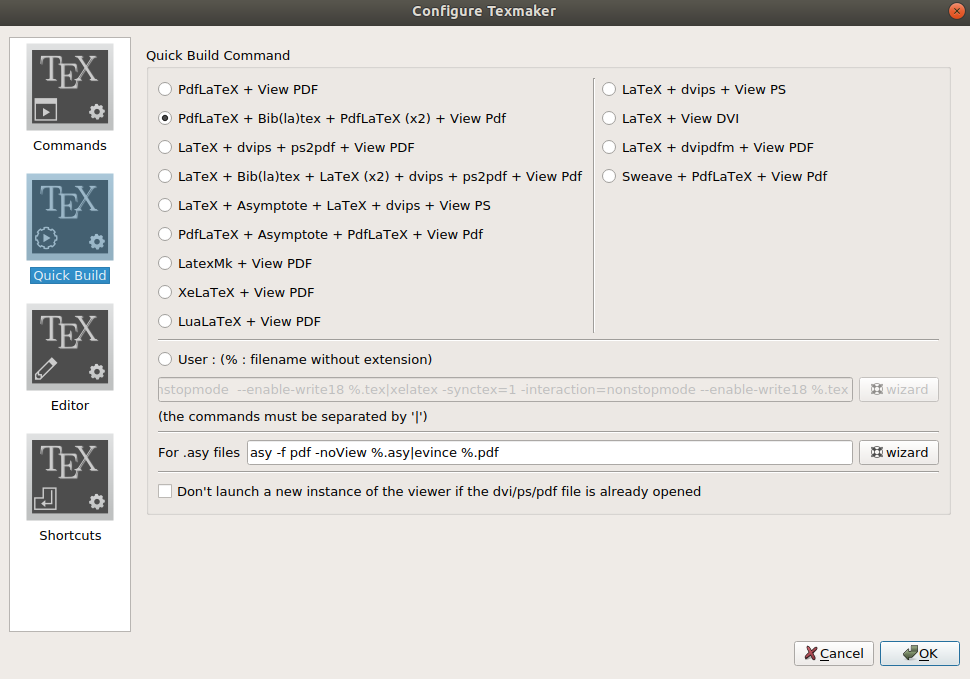
\includegraphics[width=0.8\linewidth]{figures/config-texmaker.png}
\end{center}
   \caption{Compiling this document using \emph{TexMaker}.}
\label{fig:google-scholar-2col}
\end{figure*}


\section{Motivation}

Describe why your project is interesting. E.g., you can describe how your project may have an impact. Or, you may describe the motivation from a personal learning perspective.

\section{Resources}

What tools and libraries have you used.

\section{Challenges and Problems}

Describe the technical problems you had even if you haven't managed to solve. Also describe the problems that challenged you and you could address.

\section{User manual for the system}

Steps to run your programs.


\section{Results}

Screenshots for your running programs

\section{Contributions}

You are expected to share the workload evenly, and every group member is expected to participate in both the experiments and writing.

Clearly indicate what computational and writing task each member of your group participated in.


{\small

\bibliographystyle{IEEEtran}
\bibliography{bibliography.bib}
}

\end{document}
